% Бүлэг 1

\chapter{Өгөгдөл хуваалцах үйлчилгээний тухай} % Бүлгийн нэр
\label{Chapter1} % Энэ бүлэг рүү ишлэл хийх бол \ref{Chapter1} командыг ашигла 
\pagecolor{white}
%-------------------------------------------------------------------------------

% Агуулгад ашигласан хэвшүүлэлтийн зарим командын тодорхойлолт
\newcommand{\keyword}[1]{\textbf{#1}}
\newcommand{\tabhead}[1]{\textbf{#1}}
\newcommand{\code}[1]{\texttt{#1}}
\newcommand{\file}[1]{\texttt{\bfseries#1}}
\newcommand{\option}[1]{\texttt{\itshape#1}}

%-------------------------------------------------------------------------------
%	SECTION 1
%-------------------------------------------------------------------------------

\section{Өгөгдөл хуваалцах үйлчилгээ}
Орчин үеийн мэдээллийн технологийн эрин үед байгууллагуудад мэдээлэл солилцох олон шалтгаан, хэрэгцээ байдаг - ажилчдад алсаас ажиллах боломжийг олгох, үйл ажиллагааны үр ашгийг дээшлүүлэх, эсвэл гуравдагч талын үйлдвэрлэгчидтэй хамтран ажиллах зэрэг олон шалтгаан бий.

\textbf{Өгөгдөл хуваалцах ямар технологиуд}\\
Өгөгдөл хуваалцах олон технологи байдаг. Зарим технологиудаас дурдвал.

\begin{itemize}
    \item \textbf{Өгөгдлийн агуулах (Data warehousing)} нь нэг буюу хэд хэдэн ялгаатай эх сурвалжийг нэгтэгсэн төвлөрсөн агуулах юм. Архитектур нь шатлалаас бүрддэг. Дээд давхарга нь тайлагнах, дүн шинжилгээ хийх, үр дүнг харуулдаг front-end клиент юм. Дунд шат нь өгөгдөлд хандах, дүн шинжилгээ хийхэд ашигладаг аналитик механизмаас бүрдэнэ. Доод шат нь өгөгдлийг ачаалах, хадгалах өгөгдлийн сангийн сервер юм. Дээд болон дунд түвшний програмууд нь доод давхаргад хадгалагдсан нийтлэг өгөгдлийн багцыг хуваалцах боломжтой.
    
    \item \textbf{Хэрэглээний программчлалын интерфэйс (API)} нь програм хангамжийн хоёр бүрэлдэхүүн хэсэг нь тодорхой протоколуудыг ашиглан хоорондоо харилцах боломжийг олгодог механизм юм. Интерфэйсийг  хоёр програмын хоорондох үйлчилгээний тохиролцоо гэж үзэж болно. Энэхүү тохиролцоо нь хэрхэн харилцах хүсэлт болон хариултыг тодорхойлдог. Хандалтыг нарийн тодорхойлж болдог ба хэрэглэгчид яг ямар өгөгдөл хүсч болохыг зааж өгдөг.
    
    \item \textbf{Холбооны сургалт (Federated learning)} нь тархсан өгөгдлийг багц дээр хиймэл оюун ухааныг сургах боломжийг олгодог. Бүх өгөгдлийг нэг дор цуглуулж нэгтэхийн оронд тус тусдаа төхөөрмж дээр хадгалж зөвхөн загварийн шинэчлэлтүүдийг төв сервер рүү илгээдэг.

    \item \textbf{Блокчейн технологи} нь сүлжээн дотор ил тод мэдээлэл солилцох боломжийг олгодог өгөгдлийн сангийн дэвшилтэт механизм юм. Өгөгдлийг гинжин хэлхээнд холбосон блокуудад хадгалдаг. Сүлжээнээс зөвшилцөлгүйгээр гинжийг устгах эсвэл өөрчлөх боломжгүй.

    \item \textbf{Өгөгдөл солилцох платформууд}
    
    Нээлттэй өгөгдлийн платформууд нь өөр өөр өгөгдлийн багцийг нийтийн хэрэгцээнд ашиглах боложийг ологдог. Ихэвчлэн өгөгдлийн менежмент, өгөгдлийн аюулгүй байдал, өгөгдөл нэгтгэх, өгөгдөл хуваалцах, хамтран ажиллах зэрэг олон төрлийн функцуудыг санал болгодог.
\end{itemize}

%-------------------------------------------------------------------------------
%	SECTION 2
%-------------------------------------------------------------------------------

\section{Өгөгдлийн аюулгүй байдал}

Өгөгдлийн аюулгүй байдал гэдэг нь дижитал мэдээллийг зөвшөөрөлгүй хандах, өөрчлөх, хулгайлахаас хамгаалах үйл ажиллагаа юм. Физик төхөөрөмжийн хамгаалалтаас эхлээд хандалтын удирдлаг, програм хангамжийн логик аюулгүй байдал мэдээллийн аюулгүй байдалын бүх талыг хамарсан ойлголт юм.

\textbf{Ягаад өгөгдлийн аюулгүй байдал чухал вэ?}

Таний нууц эмзэг мэдээлэл санхүүгийн чадамж бичиг баримт зэргийг буруу зорилгоор ашиглах аюултай.

Байгуулгын хувьд хэрэглэгчдийнхээ мэдээлэл өгөгдлийг алдаж буруу гарт орохоос сэргийлэж хуулийн дагуу хамгаалах ёстой. Мөн тухайн байгуулга нь хакдуулах мэдээлэлээ алдах нь нэр хүнд нь халтай ба хэрэглэгчдийн итгэлийг алдах аюултай.

\textbf{Өгөгдлийн аюулгүй байдлын төрлүүд}
\begin{itemize}
    \item \textbf{Шифрэлэлт} нь түлхүүр нууц үггүйгээр өгөгдлийг унших боломжгүй бологдог ба криптографын алгоритмуудыг ашиглан энгийн текстийг шифрлэх үйл явц юм. Энэ нь халдагчид өгөгдөлд нэвтэрсэн байсан ч зохих итгэмжлэлгүйгээр үүнийг уншиж чадахгүй гэдгийг баталгаажуулахад тусалдаг.
    \item \textbf{Хандалтын удирдлага} нь нууц өгөгдөлд хэн хандах эрхтэй болохыг тэдний үүрэг, зөвшөөрлийн түвшинд үндэслэн хязгаарладаг. Үүнд нууц үг, биометрийн баталгаажуулалт, хамгаалалтын токен зэрэг арга хэмжээ багтана.
    \item \textbf{Нөөцлөх, сэргээх} үйл явц нь аюулгүй байдлын зөрчил эсвэл өгөгдөл алдагдсан тохиолдолд сэргээх боломжтой байхын тулд мэдээллийн хуулбарыг үүсгэх, хадгалах явдал юм.
    \item \textbf{Физик аюулгүй байдал} нь өгөгдөл хадгалах төхөөрөмж болон физик хандалтыг хамгаалахын тулд түгжээтэй хаалга, хамгаалалтын камер зэрэг физик хамгаалалтын арга хэмжээг ашигладаг.
    \item \textbf{Өгөгдөл устгах} Өгөгдлийг устгах нь хамгийн аюулгүй хэдий дахин ашиглах боломжгүй. Ихэвчлэн дахин ашиглахгүй өгөгдлийн дарж бичих зэргээр устгадаг.
    \item \textbf{Өгөгдлийн далдлах} нь нууц мэдээллийг анхны өгөгдлийн бүтцийг хадгалан зөвшөөрөлгүй хэрэглэгчдэд ашиглах боломжгүй болгож буй хуурамч мэдээллээр солих явдал юм.
\end{itemize}

\textbf{Аюулгүй өгөгдөл хуваалцах}


%-------------------------------------------------------------------------------
%	SECTION 3
%-------------------------------------------------------------------------------

\section{Шифрлэх схемүүд}
Өгөгдлийг хэрхэн найдвартай нууцлаж хамгаалах нь чухал болсон. Зөвхөн шифрлэхээс гадна үүнийг схемчилж илүү хурдан өөр өөрсдийн давуу талтай схемүүдмйг хөгжүүлж гаргаж ирсэн.

\textbf{Танилтад суурилсан шифрлэлт (IBE)} 

Нийтийн түлхүүрийн оронд өөрийн хувийн мэдээллийг ашиглан өгөгдлийг шифрлэх, тайлах боломжийг олгодог нийтийн түлхүүрийн шифрлэлтийн нэг төрөл юм. IBE-ийг хэрэглэгчдийг таних тэмдэгээр нь мэддэг тохиолдолд аюулгүй өгөгдөл хуваалцахад ашиглаж болно.

\textbf{Шинж чанарт суурилсан шифрлэлэт (ABE)}

Энэ нь нас, албан тушаал, байгууллагын үүрэг зэрэг урьдчилан тодорхойлсон шинж чанарт үндэслэн өгөгдөлд хандах боломжийг олгодог шифрлэлтийн төрөл юм. ABE нь өгөгдөлд хандах хандалтыг нарийн хянахад ашиглагдаж болох ба зарим шинж чанарууд дээр үндэслэн хандалт олгосон хувилбаруудад ашиглаж болно.

\textbf{Гомоморф шифрлэлт (HE)}

Энэ нь шифрлэгдсэн өгөгдлийг эхлээд тайлахгүйгээр тооцоолол хийх боломжийг олгодог шифрлэлтийн төрөл юм. Тооцоолол хийх боломжийг олгохын зэрэгцээ өгөгдлийг нууцлах шаардлагатай тохиолдолд HE-г аюулгүй өгөгдөл боловсруулахад ашиглаж болно.

\textbf{Secure multiparty computation (MPC)}

Энэ талууд өөрсдийн оролтыг бие биедээ ил гаргахгүйгээр хувийн оролт дээрээ функцийг хамтран тооцоолох боломжийг олгодог криптографийн арга юм. Мэдээллийн нууцлалыг хадгалах, олон тал хамтран ажиллах шаардлагатай тохиолдолд MPC-ийг аюулгүй өгөгдөл боловсруулахад ашиглаж болно.

\textbf{Прокси дахин шифрлэлт (PRE)}

%-------------------------------------------------------------------------------
%	SECTION 4
%-------------------------------------------------------------------------------

\section{Файл шифрлэх аргууд}

\section{Шифрлэлт, түүний ач холбогдол, ангилал, хэрэглээ}
Мэдээллийн аюулгүй байдал үндсэн гурван зарчимыг тэнцвэртэй хангахыг зоридог. 
\begin{itemize}
    \item \textbf{Нууцлаг байдал (Confidentiality)}: Мэдээлэлийг нууц хэвээр нь хамгаалж үлдэх. Санаатай болон санамсаргүй мэдээллийг зөвшөөрөлгүй хуваалцах тараахаас сэргийлэх.
    \begin{itemize}
        \item Өгөгдлийн нууцлал (Data1 confidentiality)
        \item хувийн нууц (Privacy)
    \end{itemize}
    \item \textbf{Бүрэн бүтэн байдал (Integrity)}: Өгөгдөлд үнэн зөв найдвартай гадны нөлөө ороогүйг шалгах, бүрэн бүтэн хадаглах. 
    \begin{itemize}
        \item Өгөгдлийн бүрэн бүтэн байдал (Data integrity)
        \item Системийн бүрэн бүтэн байдал (System integrity) 
    \end{itemize}
    \item \textbf{Хүртээмжтэй байдал (Availability):} Тухайн системийн хэрэглэгчид хүртээмжтэй байх.
\end{itemize}

\begin{figure}[ht]
\centering
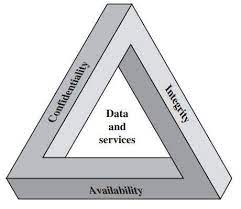
\includegraphics[scale=0.7]{Figures/cia_traid}
\caption[CIA гурвалжин]{CIA гурвалжин}
\label{fig:CIA}
\end{figure}

Криптографд шифрлэлт нь энгийн текстийг (жишээ нь, эх мессеж) шифр текст (жишээ нь, шифрлэгдсэн эсвэл кодлогдсон мессеж) болгон хувиргахад ашигладаг алгоритм юм. Шифрлэлтийн зорилго нь мессежийг түлхүүргүй хүн унших боломжгүй болгох явдал юм.

Мэдээлэл болон өгөгдлийг шифрлэлт хийснээр нууцлаг байдлыг хангах хамгийн том давуу тал юм. Бүрэн бүтэн байдал болон хүртээмжтэй байдлыг ч шифрлэлт нь хангах боломжтой.
Шифрлэлт ерөнхийд нь гурав ангилна.
\begin{itemize}
    \item \textbf{Тэгш хэмт шифрлэлт (symmetric)} нь шифрийг тайлах болон шифрлэхдээ нэг түлхүүр ашигладаг. Уламжлалт шифрлэлт гэх нь бий. Уламжлалт (компьютероос өмнөх үе) тэгш хэмтэй шифрүүд нь орлуулах эсвэл шилжүүлэх аргыг ашигладаг. Орлуулах арга нь энгийн текстийн элементүүд (тэмдэгтүүд, битүүд) шифр текстийн элементүүдэд солино оруулж тавина. Шилжүүлэх техник нь энгийн текстийн элементүүдийн байрлалыг системтэйгээр шилжүүлдэг. 
    Тэгш хэмт шифрлэлт нь хоёр төрөлтэй.
    \begin{itemize}
        \item Урсгал шифрлэлт (Stream шифрлэлт) RC4 болон ChaCha20 гэх мэт.
        \item Блок шифрлэлт (Block шифрлэлт) AES, DES, болон 3DES гэх мэт.
    \end{itemize}
    \item \textbf{Тэгш бус шифрлэлт (asymmetric)} нь нийтийн болон хувийн хоёр түлхүүртэй. Нийтийн түлхүүр нь нийтэд нээлтэй байдаг. Хувийн түлхүүрийг эмзэгшигч нь нууцалж алдахгүй байх ёстой. 
    \item \textbf{Хэш (Hash)} функц нь хувьсах урттай мессежийг тогтмол урттай хэш утга шифрлэдэг. Ихэнх хэш функц нь шахалтын алгоритм ашигладаг.
\end{itemize}

Криптограф нь дамжуулалтын явцад мессежийг хөндлөнгөөс өөрчлөлт ороогүй эсэхийг шалгаж бүрэн бүтэн байдлыг хангадаг. Хэш, мессежийг баталгаажуулалтын код (MACs), тоон гарын үсэг (Digital Signatures) ашигладаг байдаг.

\textbf{Мессежийн баталгаажуулалтын код (MACs)} нь авсан өгөгдөл нь илгээсэнтэй яг таарч (өөрчлөлт оруулах, устгах) мөн илгээгчийн баталгаажуулдаг.
Нууц түлхүүр ашигдаг. MAC нь хувьсах урттай мессежийг нууц түлхүүр болгон авч, баталгаажуулах код үүсгэдэг. MAC нь хэш функц болон тэгш хэмт блок шифрлэлтийг ашиглдаг.

\textbf{Тоон гарын үсэг (Digital Signatures)}

Ихэвчлэн шифрлэгдсэн мессэж, энгийн мессежийн хэшийг бүтээгчийн хувийн түлхүүрийн хэшийг авч харьцуулж баталгаажуулдаг.

%-------------------------------------------------------------------------------
%	SECTION 5
%-------------------------------------------------------------------------------

\section{Бүлгийн Дүгнэлт}
Энэ бүлэгт орчин үеийн шифрлэлтийн схеммүүдмйг судалж прокси дахин шифрлэлэт нь бусад схеммүүдээс ямар давуу тал сул талыг судалж харицуулсан. Системийн хөгжүүлэлт ерөнхий загварийг гаргаж юу хэрэгтэй сангуудыг ашиглан системийн хөгжүүлэлтыг хийж элсэн.